\newpage
\disableTemplate{LugatexLogo}
\disableTemplate{Navigatorbarbg}
\disableTemplate{Lugamathbg}
%
%\disableTemplate{Lugamechanicscover}
%
%\AddToTemplate{susebganim}
%\AddToTemplate{Navigatorbarbg}
%\AddToTemplate{LugatexLogo}
\begin{tikzpicture}[remember picture,overlay,cap=round]
% Local definitions
%\def\costhirty{0.8660256}
% Colors
%\colorlet{anglecolor}{green!50!black}
%\colorlet{sincolor}{red}
%\colorlet{tancolor}{orange!80!black}
%\colorlet{coscolor}{blue}
% Styles
%\tikzstyle{axes}=[]
%\tikzstyle{important line}=[very thick]
%\tikzstyle{information text}=[rounded corners,fill=red!10,inner sep=1ex]
%
%\draw (0.2,-1) circle (1cm);
%
%\begin{scope}[style=axes]
%	\draw[->] (-1.5,0) -- (1.5,0) node[right] {$x$};
%	\draw[->] (0,-1.5) -- (0,1.5) node[above] {$y$};
%	\draw[->] (-0.91,-1) -- (1.5,-1) node[right] {$x$};
%	\draw[->] (0.2,-2.2) -- (0.2,0.3) node[left] {$y$};
%	\foreach \x/\xtext in {-1, -.5/-\frac{1}{2}, 1}
%		\draw[xshift=\x cm] (0pt,1pt) -- (0pt,-1pt) node[below]
%		{$\xtext$};
%
%	\foreach \y/\ytext in {-1, -.5/-\frac{1}{2}, .5/\frac{1}{2}, 1}
%		\draw[yshift=\y cm] (1pt,0pt) -- (-1pt,0pt) node[left]
%		{$\ytext$};
%\end{scope}			
%
%\filldraw[fill=green!20,draw=anglecolor] (0,0) -- (3mm,0pt) arc(0:30:3mm);
%\draw (15:2mm) node[anglecolor] {$\alpha$};
%
%\draw[style=important line,sincolor]
%	(30:1cm) -- node[left=1pt] {$\sin \alpha$} +(0.2,-.5);
%
%\draw[style=important line,coscolor]
%	(0.2,-1) -- node[below=2pt] {$\cos \alpha$} (\costhirty,-1);
%\draw[scale=0.5,style=important line,tancolor] (1,0) -- node [right=1pt]
%{
%	$\displaystyle \tan \alpha \color{black}=
%	\frac{{\color{sincolor}\sin \alpha}}{\color{coscolor}\cos \alpha}$
%	} (intersection of 0,0--30:1cm and 1,0--1,1) coordinate (t);
%\draw (0,0) -- (t);
%
%	\node [scale=0.5,text opacity=0.99] at (current page.north) {%
%\node [scale=0.6,text opacity=0.99] at (6.7,-0.6) {%
%	$C^2 = A^2 + B^2\qquad \sin a = A/C\qquad \cos a = B/C\qquad
%		C/A\qquad \sec a = C/B$};
%\node [scale=0.95,text opacity=0.99] at (4,0) {$ \sin a = A/C, \quad
%	\cos a = B/C, \\
%	\csc a = C/A, \quad \sec a = C/B, \\$};
%\node at (0.3,-5) {\psfig{file=triangle.fig}};
%Pythagorean theorem: $ C^2 = A^2 + B^2 $
%Definitions:
%$
%\sin a = A/C, \quad
%\cos a = B/C, \\
%\csc a = C/A, \quad
%\sec a = C/B, \\
%\tan a = {\sin a \over \cos a} =  {A \over B}, \quad
%\cot a = {\cos a \over \sin a} =  {B \over A}. \\
%$
%Area, radius of inscribed circle:
%$\frac{1}{2} A B, \quad \frac{A B}{A + B + C}$
\node[scale=0.9,chamfered rectangle,white,fill=green,double=red,draw,very thick] 
	at (6.6,-9.2) { \bf АНИМАЦИЯ};
\end{tikzpicture}
%Identities:
%\vskip 3pt
%\Dis 5pt
%\baselineskip=22pt
%\Fm \sin x = {1 \over \csc x}, \Mf
%\Fm \cos x = {1 \over \sec x}, \Mf
%\Fm \tan x = {1 \over \cot x}, \Mf
%\Fm \sin^2 x + \cos^2 x = 1, \Mf
%\Fm 1 + \tan^2 x = \sec^2 x, \Mf
%\Fm 1 + \cot^2 x = \csc^2 x, \Mf
%\Fm \sin x = \cos \left(\sfrac {\pi} 2 - x\right), \Mf
%\Fm \sin x = \sin (\pi - x), \Mf
%\Fm \cos x = - \cos (\pi - x), \Mf
%\Fm \tan x = \cot \left(\sfrac {\pi} 2 - x\right), \Mf
%\Fm \cot x = - \cot (\pi - x), \Mf
%\Fm \csc x = \cot \sfrac x 2 - \cot x, \Mf
%\Fm \sin (x \pm y) = \sin x \cos y \pm \cos x \sin y, \Mf
%\Fm \cos (x \pm y) = \cos x \cos y \mp \sin x \sin y, \Mf
%\Fm \tan (x \pm y) = { \tan x \pm \tan y \over 1 \mp \tan x \tan y}, \Mf\vadjust{\kern4pt}
%\Fm \cot (x \pm y) = {\cot x \cot y \mp 1 \over \cot x \pm \cot y }, \Mf
%\Fm \sin 2 x =  2 \sin x \cos x, \Mf
%\Fm \sin 2 x = {2 \tan x \over 1 + \tan^2 x}, \Mf
%\Fm \cos 2 x = \cos^2 x  - \sin^2 x, \Mf
%\Fm \cos 2 x = 2 \cos^2 x - 1, \Mf
%\Fm \cos 2 x = 1 - 2 \sin^2 x,  \Mf
%\Fm \cos 2 x = {1 -  \tan^2 x \over 1 + \tan^2 x}, \Mf\vadjust{\kern5pt}
%\Fm \tan 2 x = {2 \tan x \over 1 - \tan^2 x}, \Mf
%\Fm \cot 2 x = {\cot^2 x - 1 \over 2 \cot x}, \Mf
%\Fm \sin (x + y) \sin (x - y) = \sin^2 x - \sin^2 y, \Mf
%\Fm \cos (x + y) \cos (x - y) = \cos^2 x - \sin^2 y. \Mf
%\EndDis
%Euler's equation:
%$$
%e^{i x} = \cos x + i \sin x, \qquad e^{i \pi} = -1.
%$$
%
\vglue 21pt
\begin{center}
%\hspace{8.5pt}
\hspace{5pt}
\begin{animateinline}[autoplay,loop]{30}
%
\whiledo{\theangle<359}{
%
    \begin{tikzpicture}
    % Axis
    \draw[thick,->,blue] (-3,0)--(3,0) node[below] {$x$}; % x axis
    \draw[thick,->,blue] (0,-3)--(0,3) node[left] {$y$}; % y axis
    \draw[red,thick] (0,0) circle (2.5cm);
    \node[red,below] at (2.6,0) {1};
    \node[red,above] at (0.1,-2.5) {1};
    %
    \draw[ultra thick,cyan] (0,0) -- (0,0 |- \theangle:2.5cm); % UpOn x axis
    \draw[ultra thick,orange] (0,0) -- (\theangle:2.5cm |- 0,0); % UpOn y axis
    %
    \draw[densely dotted,orange] (\theangle:2.5cm) -- (\theangle:2.5cm |- 0,0); % vertical line
    \draw[densely dotted,cyan] (\theangle:2.5cm) -- (0,0 |- \theangle:2.5cm); % horizontal line
    \draw[ultra thick,red,->,rotate=\theangle] (0,0) -- (2.5,0); 
    \node[red,orange,right] at (0,-3.5) 
            {\footnotesize$\cos(\theangle^{\mathrm{o}}) = \pgfmathcos{\theangle}\pgfmathresult$};
    \node[red,cyan,right] at (0,-3.1) 
            {\footnotesize$\sin(\theangle^{\mathrm{o}}) = \pgfmathsin{\theangle}\pgfmathresult$};
    \end{tikzpicture}
    %
    \stepcounter{angle}
    \ifthenelse{\theangle<359}{
            \newframe
    }{
            \end{animateinline}
    }
}
\end{center}

%%%--- \newpage
%%%--- \disableTemplate{LugatexLogo}
%%%--- \disableTemplate{Navigatorbarbg}
%%%--- \disableTemplate{susebganim}
%%%--- \AddToTemplate{Lugamathtest}
%%%--- \AddToTemplate{Navigatorbarbg}
%%%--- \AddToTemplate{LugatexLogo}
%%%--- 
%%%--- 
%%%--- \vglue 45pt
%%%--- 
%%%--- \begin{center}
%%%--- \begin{animateinline}[width=0.6\linewidth]{12}
%%%--- 
%%%--- 	\multiframe{41}{n=0+1}{
%%%--- 
%%%--- \begin{tikzpicture}
%%%--- \clip (-0.5,-1.5) rectangle (5,2);
%%%--- %--------
%%%--- \draw[thin,->] (-2mm,0) -- (5,0) node[below left] {$t$};
%%%--- \draw[thin,->] (0,-1.5) -- (0,2) node[above left,rotate=90]
%%%--- {$y=\sin(t)$};
%%%--- %--------
%%%--- \draw[dashed]  (0,0) sin (1,1) cos (2,0) sin (3,-1) cos (4,0);
%%%--- %--------
%%%--- \draw[fill=blue]    (\n/10,{sin(\n*9)}) circle (1mm);
%%%--- %--------
%%%--- \end{tikzpicture}
%%%--- }
%%%--- \end{animateinline}\\[2ex]
%%%--- 
%%%--- %\makebox[0.6\linewidth][r]{toggle frame:
%%%--- %
%%%--- %\ShowHideFrame{0}{0}{$\sin 0$}
%%%--- %\ShowHideFrame{0}{10}{$\sin \frac{\pi}{2}$}
%%%--- %\ShowHideFrame{0}{20}{$\sin \pi$}
%%%--- %\ShowHideFrame{0}{30}{$\sin \frac{3}{2}\pi$}
%%%--- %\ShowHideFrame{0}{40}{$\sin 2\pi$}}\\
%%%--- \makebox[0.6\linewidth][r]{Переход по точкам:
%%%--- \GoToFrame{0}{0}{$\sin 0$}
%%%--- \GoToFrame{0}{10}{$\sin \frac{\pi}{2}$}
%%%--- \GoToFrame{0}{20}{$\sin \pi$}
%%%--- \GoToFrame{0}{30}{$\sin \frac{3}{2}\pi$}
%%%--- \GoToFrame{0}{40}{$\sin 2\pi$}}
%%%--- 
%%%--- \end{center}
\begin{textblock}{15}(-0.6,1.9)
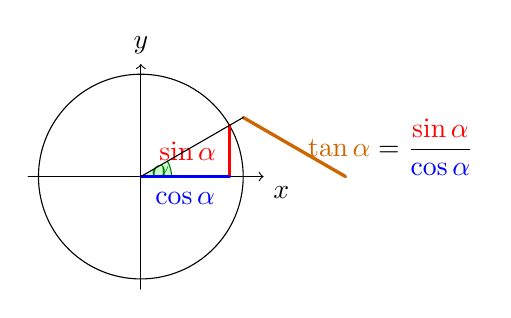
\begin{tikzpicture}[scale=1.3,cap=round]
  % Local definitions
  \def\costhirty{0.8660256}
  % Colors
  \colorlet{anglecolor}{green!50!black}
  \colorlet{sincolor}{red}
  \colorlet{tancolor}{orange!80!black}
  \colorlet{coscolor}{blue}

  % Styles
  \tikzstyle{axes}=[]
  \tikzstyle{important line}=[very thick]
  \tikzstyle{information text}=[rounded corners,fill=red!10,inner sep=1ex]

  % The graphic
  %\draw[style=help lines,step=0.5cm] (-1.4,-1.4) grid (1.4,1.4);

  \draw (0,0) circle (1cm);

  \begin{scope}[style=axes]
    \draw[->] (-1.1,0) -- (1.2,0) node[below right] {$x$};
    \draw[->] (0,-1.1) -- (0,1.1) node[above] {$y$};

%    \foreach \x/\xtext in {-1, -.5/-\frac{1}{2}, 1}
%      \draw[xshift=\x cm] (0pt,1pt) -- (0pt,-1pt) node[below]
%            {$\xtext$};
%
%   \foreach \y/\ytext in {-1, -.5/-\frac{1}{2}, .5/\frac{1}{2}, 1}
%     \draw[yshift=\y cm] (1pt,0pt) -- (-1pt,0pt) node[left]
%            {$\ytext$};
  \end{scope}

  \filldraw[fill=green!20,draw=anglecolor] (0,0) -- (3mm,0pt) arc(0:30:3mm);
  \draw (15:2mm) node[anglecolor] {$\alpha$};

  \draw[style=important line,sincolor]
    (30:1cm) -- node[left=1pt] {$\sin \alpha$} +(0,-.5);

  \draw[style=important line,coscolor]
    (0,0) -- node[below=2pt] {$\cos \alpha$} (\costhirty,0);

  \draw[style=important line,tancolor] (2,0) --
    node [right=1pt]
    {
      $\displaystyle \tan \alpha \color{black}=
      \frac{{\color{sincolor}\sin \alpha}}{\color{coscolor}\cos \alpha}$
    } (intersection of 0,0--30:1cm and 1,0--1,1) coordinate (t);

  \draw (0,0) -- (t);
\end{tikzpicture}
\end{textblock}	 

